%!TEX TS-program = xelatex
\documentclass[10pt,oneside]{article}
\usepackage[fontsize=9pt]{scrextend}

\usepackage[english]{babel}

\usepackage{amsmath,amssymb,amsfonts}
\usepackage[utf8]{inputenc}
\usepackage[T1]{fontenc}
\usepackage{stix2}
\usepackage[scaled]{helvet}
\usepackage[scaled]{inconsolata}

\usepackage{lastpage}

\usepackage{setspace}

\usepackage{ccicons}

\usepackage[hang,flushmargin]{footmisc}

\usepackage{geometry}

\setlength{\parindent}{0pt}
\setlength{\parskip}{6pt plus 2pt minus 1pt}

\usepackage{fancyhdr}
\renewcommand{\headrulewidth}{0pt}\providecommand{\tightlist}{%
  \setlength{\itemsep}{0pt}\setlength{\parskip}{0pt}}

\makeatletter
\newcounter{tableno}
\newenvironment{tablenos:no-prefix-table-caption}{
  \caption@ifcompatibility{}{
    \let\oldthetable\thetable
    \let\oldtheHtable\theHtable
    \renewcommand{\thetable}{tableno:\thetableno}
    \renewcommand{\theHtable}{tableno:\thetableno}
    \stepcounter{tableno}
    \captionsetup{labelformat=empty}
  }
}{
  \caption@ifcompatibility{}{
    \captionsetup{labelformat=default}
    \let\thetable\oldthetable
    \let\theHtable\oldtheHtable
    \addtocounter{table}{-1}
  }
}
\makeatother

\usepackage{array}
\newcommand{\PreserveBackslash}[1]{\let\temp=\\#1\let\\=\temp}
\let\PBS=\PreserveBackslash

\usepackage[breaklinks=true]{hyperref}
\hypersetup{colorlinks,%
citecolor=blue,%
filecolor=blue,%
linkcolor=blue,%
urlcolor=blue}
\usepackage{url}

\usepackage{caption}
\setcounter{secnumdepth}{0}
\usepackage{cleveref}

\usepackage{graphicx}
\makeatletter
\def\maxwidth{\ifdim\Gin@nat@width>\linewidth\linewidth
\else\Gin@nat@width\fi}
\makeatother
\let\Oldincludegraphics\includegraphics
\renewcommand{\includegraphics}[1]{\Oldincludegraphics[width=\maxwidth]{#1}}

\usepackage{longtable}
\usepackage{booktabs}

\usepackage{color}
\usepackage{fancyvrb}
\newcommand{\VerbBar}{|}
\newcommand{\VERB}{\Verb[commandchars=\\\{\}]}
\DefineVerbatimEnvironment{Highlighting}{Verbatim}{commandchars=\\\{\}}
% Add ',fontsize=\small' for more characters per line
\usepackage{framed}
\definecolor{shadecolor}{RGB}{248,248,248}
\newenvironment{Shaded}{\begin{snugshade}}{\end{snugshade}}
\newcommand{\KeywordTok}[1]{\textcolor[rgb]{0.13,0.29,0.53}{\textbf{#1}}}
\newcommand{\DataTypeTok}[1]{\textcolor[rgb]{0.13,0.29,0.53}{#1}}
\newcommand{\DecValTok}[1]{\textcolor[rgb]{0.00,0.00,0.81}{#1}}
\newcommand{\BaseNTok}[1]{\textcolor[rgb]{0.00,0.00,0.81}{#1}}
\newcommand{\FloatTok}[1]{\textcolor[rgb]{0.00,0.00,0.81}{#1}}
\newcommand{\ConstantTok}[1]{\textcolor[rgb]{0.00,0.00,0.00}{#1}}
\newcommand{\CharTok}[1]{\textcolor[rgb]{0.31,0.60,0.02}{#1}}
\newcommand{\SpecialCharTok}[1]{\textcolor[rgb]{0.00,0.00,0.00}{#1}}
\newcommand{\StringTok}[1]{\textcolor[rgb]{0.31,0.60,0.02}{#1}}
\newcommand{\VerbatimStringTok}[1]{\textcolor[rgb]{0.31,0.60,0.02}{#1}}
\newcommand{\SpecialStringTok}[1]{\textcolor[rgb]{0.31,0.60,0.02}{#1}}
\newcommand{\ImportTok}[1]{#1}
\newcommand{\CommentTok}[1]{\textcolor[rgb]{0.56,0.35,0.01}{\textit{#1}}}
\newcommand{\DocumentationTok}[1]{\textcolor[rgb]{0.56,0.35,0.01}{\textbf{\textit{#1}}}}
\newcommand{\AnnotationTok}[1]{\textcolor[rgb]{0.56,0.35,0.01}{\textbf{\textit{#1}}}}
\newcommand{\CommentVarTok}[1]{\textcolor[rgb]{0.56,0.35,0.01}{\textbf{\textit{#1}}}}
\newcommand{\OtherTok}[1]{\textcolor[rgb]{0.56,0.35,0.01}{#1}}
\newcommand{\FunctionTok}[1]{\textcolor[rgb]{0.00,0.00,0.00}{#1}}
\newcommand{\VariableTok}[1]{\textcolor[rgb]{0.00,0.00,0.00}{#1}}
\newcommand{\ControlFlowTok}[1]{\textcolor[rgb]{0.13,0.29,0.53}{\textbf{#1}}}
\newcommand{\OperatorTok}[1]{\textcolor[rgb]{0.81,0.36,0.00}{\textbf{#1}}}
\newcommand{\BuiltInTok}[1]{#1}
\newcommand{\ExtensionTok}[1]{#1}
\newcommand{\PreprocessorTok}[1]{\textcolor[rgb]{0.56,0.35,0.01}{\textit{#1}}}
\newcommand{\AttributeTok}[1]{\textcolor[rgb]{0.77,0.63,0.00}{#1}}
\newcommand{\RegionMarkerTok}[1]{#1}
\newcommand{\InformationTok}[1]{\textcolor[rgb]{0.56,0.35,0.01}{\textbf{\textit{#1}}}}
\newcommand{\WarningTok}[1]{\textcolor[rgb]{0.56,0.35,0.01}{\textbf{\textit{#1}}}}
\newcommand{\AlertTok}[1]{\textcolor[rgb]{0.94,0.16,0.16}{#1}}
\newcommand{\ErrorTok}[1]{\textcolor[rgb]{0.64,0.00,0.00}{\textbf{#1}}}
\newcommand{\NormalTok}[1]{#1}

\newlength{\cslhangindent}
\setlength{\cslhangindent}{1.5em}
\newlength{\csllabelwidth}
\setlength{\csllabelwidth}{3em}
\newenvironment{CSLReferences}[3] % #1 hanging-ident, #2 entry spacing
 {% don't indent paragraphs
  \setlength{\parindent}{0pt}
  % turn on hanging indent if param 1 is 1
  \ifodd #1 \everypar{\setlength{\hangindent}{\cslhangindent}}\ignorespaces\fi
  % set entry spacing
  \ifnum #2 > 0
  \setlength{\parskip}{#2\baselineskip}
  \fi
 }%
 {}
\usepackage{calc} % for \widthof, \maxof
\newcommand{\CSLBlock}[1]{#1\hfill\break}
\newcommand{\CSLLeftMargin}[1]{\parbox[t]{\maxof{\widthof{#1}}{\csllabelwidth}}{#1}}
\newcommand{\CSLRightInline}[1]{\parbox[t]{\linewidth}{#1}}
\newcommand{\CSLIndent}[1]{\hspace{\cslhangindent}#1}\usepackage[table,dvipsnames]{xcolor}

\geometry{includemp,
            letterpaper,
            top=2.4cm,
            bottom=2.4cm,
            left=1.0cm,
            right=1.0cm,
            marginparwidth=5cm,
            marginparsep=1.0cm}

\usepackage[singlelinecheck=off]{caption}

\captionsetup{
  font={small},
  labelfont={bf},
  format=plain,
  labelsep=quad
}

\usepackage{floatrow}

\floatsetup[figure]{margins=hangright,
              facing=no,
              capposition=beside,
              capbesideposition={center,outside},
              floatwidth=\textwidth}

% \floatsetup[table]{margins=hangright,
%              facing=no,
%              capposition=beside,
%              capbesideposition={center,outside},
%              floatwidth=\textwidth}

\pagestyle{plain}

\setcounter{secnumdepth}{5}

\usepackage{titlesec}

\titleformat{\section}[block]
{\normalfont\large\sffamily}
{\thesection}{.5em}{\titlerule\\[.8ex]\bfseries}

\titleformat{\subsection}[runin]
{\normalfont\fontseries{b}\selectfont\filright\sffamily}
{\thesubsection.}{.5em}{}

\titleformat{\subsubsection}[runin]
{\normalfont\itshape\rmfamily\bfseries}{\thesubsubsection}{1em}{}

\fancypagestyle{firstpage}
{
   \fancyhf{}
   \renewcommand{\headrulewidth}{0pt}
   \fancyfoot[R]{\footnotesize\ccby}
   \fancyfoot[L]{\footnotesize\sffamily\today}
}

\fancypagestyle{normal}
{
  \fancyhf{}
  \fancyfoot[R]{\footnotesize\sffamily\thepage\ of \pageref*{LastPage}}
}

\usepackage{tikz}
\begin{document}
\tikz [remember picture, overlay] %
\node [shift={(-0.6in,1.1cm)},scale=0.2,opacity=0.4] at (current page.south east)[anchor=south east]{
\includegraphics{logo}};%
\pagestyle{normal}
\thispagestyle{firstpage}

\newcommand{\colorRule}[3][black]{\textcolor[HTML]{#1}{\rule{#2}{#3}}}

\noindent {\LARGE \textbf{\textsf{Solving the \(n\)-language problem: A
ecologist's guide to learning Julia}}}

\medskip
\begin{flushleft}
{\small
%
\href{https://orcid.org/0000-0002-6506-6487}{Michael D.\,Catchen}%
%
\,\textsuperscript{1,2}, %
\href{https://orcid.org/0000-0002-0735-5184}{Timothée\,Poisot}%
%
\,\textsuperscript{3,2}
\vskip 1em
\textsuperscript{1}\,McGill University; \textsuperscript{2}\,Québec
Centre for Biodiversity Sciences; \textsuperscript{3}\,Université de
Montréal\\
\vskip 1em
\textbf{Correspondance to:}\\
Michael D. Catchen --- \texttt{michael.catchen@mcgill.ca}\\
}
\end{flushleft}

\vskip 2em
\makebox[0pt][l]{\colorRule[CCCCCC]{2.0\textwidth}{0.5pt}}
\vskip 2em
\noindent

\marginpar{\vskip 1em\flushright
{\small{\bfseries Keywords}:\par
computational ecology\\scientific computing\\machine learning\\numerical
ecology\\}
}


Julia is a good language, ecologists should learn it.




\vskip 2em
\makebox[0pt][l]{\colorRule[CCCCCC]{2.0\textwidth}{0.5pt}}
\vskip 2em

\hypertarget{outline}{%
\section{Outline}\label{outline}}

\begin{itemize}
\tightlist
\item
  Why should ecologists learn julia?

  \begin{itemize}
  \tightlist
  \item
    Well, there are the criteria that are directly measureble that make
    it better than R/Python:

    \begin{itemize}
    \tightlist
    \item
      fast
    \item
      native support on GPUs
    \end{itemize}
  \item
    But there are also criteria that are more subjective, and that take
    experience and practice using the language to appreciate

    \begin{itemize}
    \tightlist
    \item
      clever use of dispatch patterns
    \item
      use of one-lienrs
    \item
      using parameterized types well
    \end{itemize}
  \item
    You will learn how to be a better programmer in \emph{any} language,
    because smart use of julia requires understanding some fundemantal
    concepts in programming that are `hidden' from users in R/python
  \item
    The biggest reason \emph{not} to use julia is that the
    ecology/evolution package ecosystem in R is larger, and the ML
    ecosystem in python is more popular. However:

    \begin{itemize}
    \tightlist
    \item
      you can call \emph{any} R/python function/library using
      RCall/PyCall in julia
    \item
      More packages isn't necessarily better when they don't work
      together
    \end{itemize}
  \end{itemize}
\end{itemize}

\begin{center}\rule{0.5\linewidth}{0.5pt}\end{center}

\hypertarget{abstract}{%
\section{Abstract}\label{abstract}}

\begin{center}\rule{0.5\linewidth}{0.5pt}\end{center}

\hypertarget{introduction}{%
\section{Introduction}\label{introduction}}

In order to measure, understand, and mitigate the consequences of
anthropogenic change on ecosystems the serives they provide, ecologists
need a set of computational tools (Urban \emph{et al.} 2022). These
tools must be performant, but crucially modular and interfaceable
(McIntire \emph{et al.} 2022).

Ecological data is often difficult to access and reuse (Gonzalez \&
Peres-Neto 2015; Poisot \emph{et al.} 2019). Many sources of ecological,
evolutionary, and environmental data exist, but synthesizing this data
into a single product suitable for analysis often remains tedious as
data are not in formats that can be easily combined or interfaced. Here
we propose that we can solve this problem through standardization
(Zimmerman 2008)---developing a common definition such that data
collected in a variety of contexts can be assimilated while minimizing
the overhead of data cleaning and wrangling.

A common representation of ecological data will have three primary
benefits: it will \textbf{1}) enable new forms of analysis by making it
easier to combine data from different sources (Heberling \emph{et al.}
2021), \textbf{2)} enable continuous integration of new data for
next-generation biodiversity monitoring (Kühl \emph{et al.} 2020), and
\textbf{3)} aid in open sharing and reproducability of published results
(Zimmerman 2008; Borregaard \& Hart 2016). Here, we briefly review
approaches to data standardization developed in other fields, in order
to determine what makes an open standard succeed in promoting data
sharing, and what doesn't. Based on the properties of good standards we
identify, we propose building a living standard for ecological data in
the \texttt{Julia} programming language, and argue this is necessary to
obtain the three primary benefits of standardization mentioned earlier.

The so-called ``two-language problem'' in computational science, where
it is easier for a researcher to developer a prototype of a
model/simulation in a high-level language, like Python or R, and later
have to port the model to a lower-level compiled language because the
performance of these compiled languages (e.g.~C++/Fortran) is orders of
magnitude faster than high level interpreted languages. In fact, many of
the most popular tools in higher-level languages are actually thin
wrappers around a compiled (often C++) base (e.g. tidyverse, keras,
numpy, TensorFlow, scikit-learn, pandas, etc.). However, the skills
required to use or debug---let alone write---scientific software in
these lower level langauges is not often taught.

We propose that that Julia has certain properties absent in other
popular languages for scientific computing that make it particularly
suited for the development of a cohesive, modular, and extendible set of
tools ideal for the development of a platform for ecological analysis
{[}@{]}.

\hypertarget{the-nature-of-computation-in-julia}{%
\section{The nature of computation in
Julia}\label{the-nature-of-computation-in-julia}}

\begin{figure}
\centering
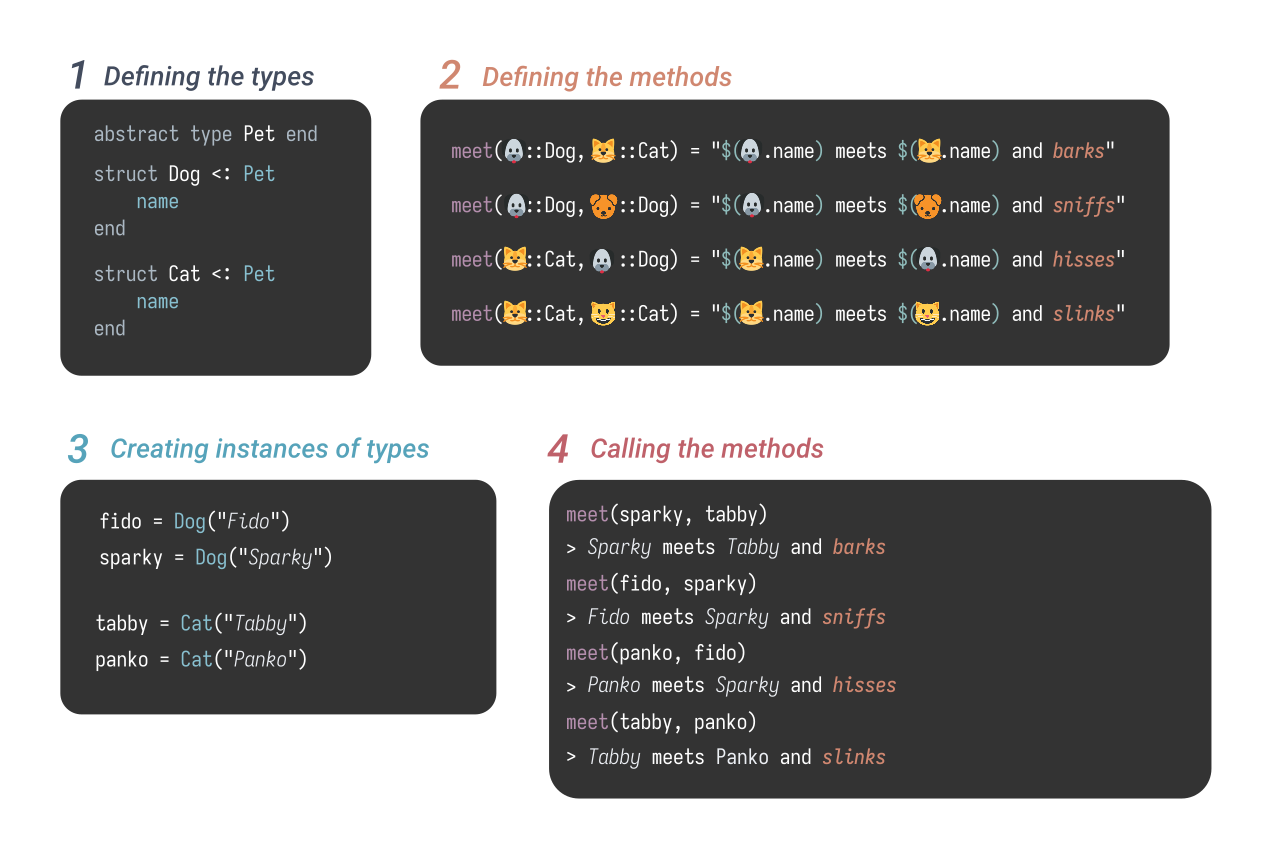
\includegraphics{./figures/multiple_dispatch.png}
\caption{TODO: caption. Adapted from Karpinski 2019 ``The unreasonable
effectiveness of multiple dispatch''}
\end{figure}

\hypertarget{types}{%
\subsection{Types}\label{types}}

Why is this useful for ecologists? Often times in ecology, the same
information is represented in different formats. Two packages in R might
not agree on what the ``correct'' format to represent information is.

At the core of the Julia language is its \emph{type system}. Type
systems can often be alienating to those who learned programming in
so-called \emph{dynamically} typed languages (like R, python, and
JavaScript). In dynamically-typed languages, \texttt{x=\ 5}, and
\texttt{x\ =\ "hello\ world"} and the language won't care that you
changed the type of information that was stored in \texttt{x} from a
number to a string. Practically, this form of dynamic-typing was adopted
because it is far more convenient to write code like that above than
defining variables with explicit types, e.g.~how you would in C:
\texttt{char\ c\ =\ "a";} and \texttt{int\ x\ =\ 5;}.

Julia doesn't require explicit type declarations, meaning
\texttt{x\ =\ 5} is perfectly valid code, but internallyJulia is doing
the bookkeeping of what type of information is stored in \texttt{x},
from an \texttt{Int64} to a \texttt{String} in the above example.

Using explicit types is central to Julia's speed, but also enables much
of its most unique and user-friendly functionality, primarily the use of
a \emph{multiple-dispatch} system.

\hypertarget{dispatch}{%
\subsection{Dispatch}\label{dispatch}}

\emph{Dispatch} refers to the way a computer program decides what
function to call.

In many staticly-typed languages, you are allow to use the same function
name more than once.

\hypertarget{doing-computational-science-in-julia}{%
\section{\texorpdfstring{Doing computational science in
\texttt{Julia}}{Doing computational science in Julia}}\label{doing-computational-science-in-julia}}

\hypertarget{managing-data}{%
\subsection{Managing Data}\label{managing-data}}

DataFrames.jl and DFMeta.

\hypertarget{doing-statistics-and-machine-learning}{%
\subsection{Doing statistics and machine
learning}\label{doing-statistics-and-machine-learning}}

\begin{enumerate}
\def\labelenumi{\arabic{enumi}.}
\setcounter{enumi}{6}
\tightlist
\item
  Learn about the statistics ecosystem: StatsBase, Statistics, GLM, MLJ,
  Flux, Turing
\end{enumerate}

\hypertarget{doing-simulation}{%
\subsection{Doing simulation}\label{doing-simulation}}

\begin{enumerate}
\def\labelenumi{\arabic{enumi}.}
\setcounter{enumi}{7}
\tightlist
\item
  Learn about the simulation libraries (DiffEq, DynamicGrids)
\item
  Learn how various statistics/simulation libraries work togethe
\end{enumerate}

\hypertarget{discussion}{%
\section{Discussion}\label{discussion}}

Defining a living standard for ecological data in \texttt{Julia} will
make it easier to combine data from different sources by splitting the
process of data aggregation from the process of analysis. Integrating
data from a particular study, or a new database, would be as simple as
implementing the interface from the data source to the standardized
types. Data from individual studies could be incorporated into public
repositories containing both the raw data and the interface to Julia
data structures, and this combined data/interface package is all that is
needed to either reproduce the results or incorporate that particular
study's data into analysis. This will make combining data from multiple
sources easier, and yield benefits for the development and
implementation of novel methods, as the software for analysis becomes
separate from the software for data cleaning and aggregation.

We envision a modern set of tools for ecology in \texttt{Julia} based
around the standardized types. Far outside of ecology, the term
``ecosystem'' is used metaphorically to describe a set of software tools
that work together. We imagine multiple ``trophic-levels'' of packages
for ecological science in \texttt{Julia} based around the ``basal'' set
of standardized types --- a modular set of tools that can be chained
together create arbitrarily complex analysis pipelines. that can be
scaled to meet the needs of next-generation biodiversity monitoring.

\hypertarget{refs}{}
\begin{CSLReferences}{1}{0}
\leavevmode\hypertarget{ref-Borregaard2016MorRep}{}%
Borregaard, M.K. \& Hart, E.M. (2016). Towards a more reproducible
ecology. \emph{Ecography}, 39, 349--353.

\leavevmode\hypertarget{ref-Gonzalez2015ActSta}{}%
Gonzalez, A. \& Peres-Neto, P.R. (2015). Act to staunch loss of research
data. \emph{Nature}, 520, 436--436.

\leavevmode\hypertarget{ref-Heberling2021DatInt}{}%
Heberling, J.M., Miller, J.T., Noesgaard, D., Weingart, S.B. \& Schigel,
D. (2021). Data integration enables global biodiversity synthesis.
\emph{Proceedings of the National Academy of Sciences}, 118.

\leavevmode\hypertarget{ref-Kuhl2020EffBio}{}%
Kühl, H.S., Bowler, D.E., Bösch, L., Bruelheide, H., Dauber, J.,
Eichenberg, David., \emph{et al.} (2020). Effective Biodiversity
Monitoring Needs a Culture of Integration. \emph{One Earth}, 3,
462--474.

\leavevmode\hypertarget{ref-McIntire2022PerRei}{}%
McIntire, E.J.B., Chubaty, A.M., Cumming, S.G., Andison, D., Barros, C.,
Boisvenue, C., \emph{et al.} (2022). PERFICT: A Re-imagined foundation
for predictive ecology. \emph{Ecology Letters}, 25, 1345--1351.

\leavevmode\hypertarget{ref-Poisot2019EcoDat}{}%
Poisot, T., Bruneau, A., Gonzalez, A., Gravel, D. \& Peres-Neto, P.
(2019). Ecological Data Should Not Be So Hard to Find and Reuse.
\emph{Trends in Ecology \& Evolution}, 34, 494--496.

\leavevmode\hypertarget{ref-Urban2022CodLif}{}%
Urban, M.C., Travis, J.M.J., Zurell, D., Thompson, P.L., Synes, N.W.,
Scarpa, A., \emph{et al.} (2022). Coding for Life: Designing a Platform
for Projecting and Protecting Global Biodiversity. \emph{BioScience},
72, 91--104.

\leavevmode\hypertarget{ref-Zimmerman2008NewKno}{}%
Zimmerman, A.S. (2008). New Knowledge from Old Data: The Role of
Standards in the Sharing and Reuse of Ecological Data. \emph{Science,
Technology, \& Human Values}, 33, 631--652.

\end{CSLReferences}

\end{document}
